\section{Aufbau}
\label{sec:Aufbau}

Zur Bestimmung der effektiven Masse der Leitungselektronen von n-dotierten Gallium Arsenid, wird die Faraday Rotation
gemessen. Dabei wird der in \ref{fig:apparatur} dargestellte Versuchaufbau verwendet.

\begin{figure}[H]
    \centering
    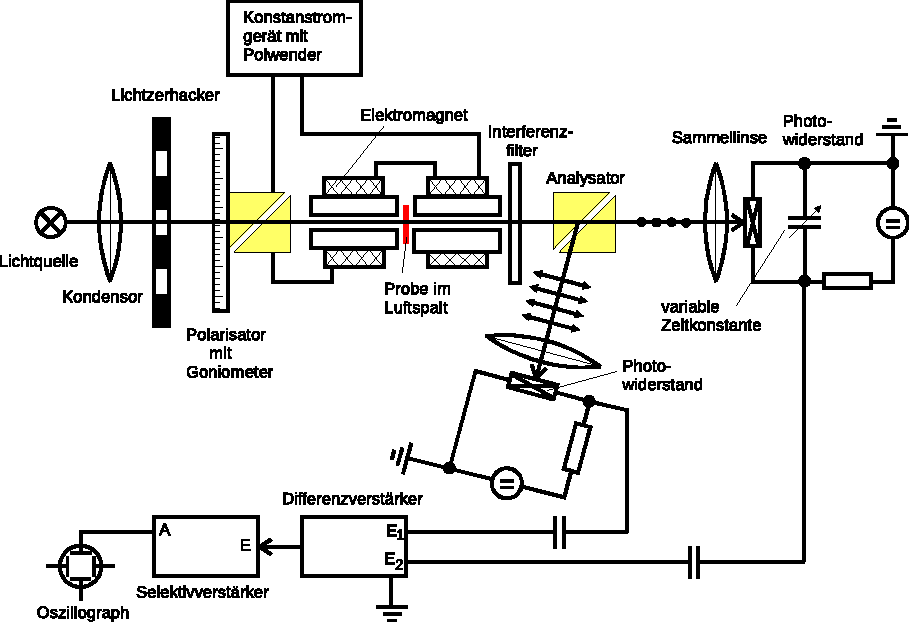
\includegraphics[width=0.8\textwidth]{content/grafik/apparatur.pdf}
    \caption{Schematische Darstellung der Messapparatur. \cite{faraday}}
    \label{fig:apparatur}
\end{figure}

Die Halogenlampe besitzt ein Emessionsspektrum im hauptsächlich Infrarotbereich. Dieses Licht trifft auf einen
Sammellinse, so dass das Licht parallelisiert wird und anschließend durch einen Licht-Zerhacker gepulst wird.
Das nun gepulste Licht trifft senkrecht auf ein Glan Thomson Prisma, welche anhand eines Goniometer drehbar gelagert ist.
Sobald der Lichtstrahl aus dem Prisma austritt, ist dieses linear polarisiert. Mit Hilfe des Gonimeters lässt sich 
der Polarisationswinkel ablesen. 

Unsere scheibenförmige Probe befindet sich in einem Elektromagneten, welcher durch ein Konstantstromgerät gespeist wird.
So ist die Probe mit eionem zeitlich Konstanten Magnetfeld durchsetzt.
Das linear polariserte Licht durchqueert den Elektromagenten und die verwendete Probe.
Im Anschluss trifft der Lichtstrahl auf einen Interferenzfilter und wird so monchromatisert.
Das nahezu monochromatische Licht fällt auf einen zweiten Glan Thomson Prisma und wird demnach
zu einen ordentlichen und außerordentlichen Lichtstrahl geteilt. Die Lichtstrahlen sind orthogonal zueinander linear polarisiert.
Die Strahlen treffen darauf jeweils auf einen Photowiderstand.

